% Module D: The Roadmap
% INStats Data Can Deceive: Causal Roadmaps with (and without) AI workshop
% August 5, 2026 | 1:35--2:20 ET | Andy Wilson
%
% BUILD: compile TWICE (or latexmk -pdf). This deck uses tikz
% [remember picture] overlays; a single fresh pass misplaces the
% title slide, band tags, and footer.
\documentclass[aspectratio=169]{beamer}

% ==================== Theme and packages ============================
\usetheme{metropolis}
\usefonttheme{professionalfonts}
\usepackage[utf8]{inputenc}
\usepackage{amsmath, amssymb}
\usepackage{graphicx}
\usepackage{lmodern}
\usepackage{microtype}
\usepackage{xcolor}
\usepackage{tikz}
\usetikzlibrary{calc}

% ==================== Palette and chrome ============================
\definecolor{accent}{HTML}{4A9EFF}
\definecolor{slate}{HTML}{23373B}   % metropolis mDarkTeal; header band

\setbeamercolor{structure}{fg=accent}
\setbeamercolor{background canvas}{bg=white}
\setbeamercolor{alerted text}{fg=accent}
% fg = bg turns metropolis's growing progress bar into a constant
% full-width accent rule under the title band.
\setbeamercolor{progress bar}{fg=accent, bg=accent}
\setbeamerfont{frametitle}{series=\bfseries}
\metroset{progressbar=frametitle, block=fill}
\setbeamertemplate{navigation symbols}{}
\makeatletter
\setlength{\metropolis@progressinheadfoot@linewidth}{1.6pt}
\makeatother

% No footer on this deck: the slides are dense and were written to use
% the full frame height; the header band carries the format.
\setbeamertemplate{footline}{}
% ====================================================================

\title{The Causal Roadmap}
\subtitle{Data Can Deceive: Causal Roadmaps with (and without) AI}
\author{Andy Wilson}
\institute{Module D: The Roadmap}
\date{August 5, 2026 \quad $\cdot$ \quad 1:35--2:20 ET}

\begin{document}

% --------------------------------------------------------------------
% Title
% --------------------------------------------------------------------
\begin{frame}[plain]
  \begin{tikzpicture}[remember picture,overlay]
    \node[anchor=north east]
      at ([xshift=-0.6cm,yshift=-0.5cm]current page.north east)
      {
\includegraphics[width=2.9cm]{art/InStats_RWL.png}};

    \node[anchor=west, text=slate,
          font=\bfseries\fontsize{27}{31}\selectfont]
      at ([xshift=1.4cm,yshift=1.55cm]current page.west)
      {The Causal Roadmap};
    \node[anchor=west, text=accent, font=\fontsize{14.5}{18}\selectfont]
      at ([xshift=1.42cm,yshift=0.72cm]current page.west)
      {Data Can Deceive: Causal Roadmaps with (and without) AI};

    \draw[black!16, line width=0.5pt]
      ([xshift=1.42cm,yshift=0.05cm]current page.west) --
      ([xshift=7.6cm,yshift=0.05cm]current page.west);

    \node[anchor=west, text=slate,
          font=\bfseries\fontsize{10.5}{13}\selectfont]
      at ([xshift=1.42cm,yshift=-0.62cm]current page.west)
      {Module D \(\cdot\) The Roadmap};
    \node[anchor=west, text=black!55, font=\fontsize{9.5}{12}\selectfont]
      at ([xshift=1.42cm,yshift=-1.18cm]current page.west)
      {August 5, 2026 \(\cdot\) 1:35--2:20 ET};

    \node[anchor=west, text=black!60, font=\fontsize{9.5}{12}\selectfont]
      at ([xshift=1.42cm,yshift=-2.35cm]current page.west)
      {Andy Wilson};
  \end{tikzpicture}
\end{frame}

% --------------------------------------------------------------------
\begin{frame}{Overview: The Causal Roadmap}
  \small
  \textbf{This module covers:}
  \begin{itemize}
    \item A target-trial protocol that fixes the question and time zero
    \item The 9-step literature version of the Causal Roadmap
    \item A worked example: pneumococcal vaccine and pneumonia
    \item How nine literature steps map to eight Causal Navigator steps
  \end{itemize}
  \vspace{0.4em}
  \textbf{Key takeaway:} The roadmap surfaces assumptions \textbf{before}
  touching data $\rightarrow$ separating design from analysis.

  \vspace{0.4em}
  {\scriptsize\color{black!55}Step counts vary across the literature
  (7--9 depending on grouping). We teach the nine-step literature sequence,
  then show how Navigator groups the same work into eight operational steps.\par}
\end{frame}

\section{Why a Roadmap?}

\begin{frame}{Surface assumptions before analysis}

\begin{figure}
	\centering
	\includegraphics[height=0.75\textheight,keepaspectratio]{art/iceberg}
\end{figure}


\end{frame}

% ----------------------------------------
\begin{frame}{The Challenge: Rigorous Causal Inference from RWD}
  \small
  \textbf{Real-world data (RWD) is abundant but messy:}
  \begin{itemize}
    \item But as we saw, data can be deceptive (without a roadmap)
    \item Treatment decisions are \emph{not} randomized
    \item Confounding, selection bias, and measurement error abound
  \end{itemize}
  \vfill
  \textbf{The fundamental problem:}
  \begin{center}
    \Large How do we draw \textbf{causal} conclusions from \textbf{observational} data?
  \end{center}
  \vfill
  \textcolor{accent}{\textbf{Solution:}} A structured framework that makes assumptions \textbf{explicit}, decisions \textbf{transparent}, and limitations \textbf{honest :)}
\end{frame}

% ----------------------------------------
\begin{frame}{Motivating Example: Pneumococcal Vaccine}
  \small
  \setlength{\abovedisplayskip}{5pt}\setlength{\belowdisplayskip}{5pt}
  \textbf{Question:} Does the pneumococcal vaccine reduce pneumonia risk (hospitalization for pneumonia)?
  \vspace{0.25em}

  \textbf{Observed pattern in the teaching data:}
  \begin{itemize}
    \item People with higher baseline risk are more likely to be vaccinated
    \item Age and prior pneumonia predict hospitalization risk
  \end{itemize}
  \vspace{0.25em}

  \textbf{A na\"ive comparison often shows:}
  \[
    \text{Risk of pneumonia among vaccinated} \;>\; \text{Risk among unvaccinated}
  \]
  \vspace{0.25em}

  \textcolor{red}{\textbf{Interpretation error:}} Treating the observed association as causal.
  \vspace{0.25em}

  \textcolor{accent}{\textbf{What went wrong?}} Without a causal model, we confuse association with causation. We need the Causal Roadmap.
\end{frame}

\section{Target Trial Emulation}

% ----------------------------------------
\begin{frame}{Target Trial Emulation: Thinking Like an Experimenter}
  \small
  \textbf{Key insight:} Design observational studies as if planning an RCT (Hern{\'a}n \& Robins, 2016)
  \vspace{0.5em}

  \begin{columns}[T]
    \begin{column}{0.46\textwidth}
      \textbf{Target Trial Protocol:}
      \begin{itemize}
        \item Eligibility criteria
        \item Treatment strategies
        \item Treatment assignment
        \item Outcome definition
        \item Follow-up period
        \item Causal contrast
      \end{itemize}
    \end{column}
    \begin{column}{0.46\textwidth}
      \textbf{Emulation in RWD:}
      \begin{itemize}
        \item Define inclusion/exclusion
        \item Specify interventions
        \item Identify time zero
        \item Operationalize outcome
        \item Set observation window
        \item Choose effect measure
      \end{itemize}
    \end{column}
  \end{columns}
  \vspace{0.5em}

  \textcolor{red}{\textbf{Critical:}} Align \textbf{eligibility}, \textbf{treatment assignment}, and \textbf{follow-up start} at time zero.
  \vspace{0.3em}

  {\footnotesize Misalignment causes immortal time bias, selection bias, and other systematic errors.}
\end{frame}

\begin{frame}{The Causal Roadmap: A 9-Step Framework}

\begin{figure}
	\centering
	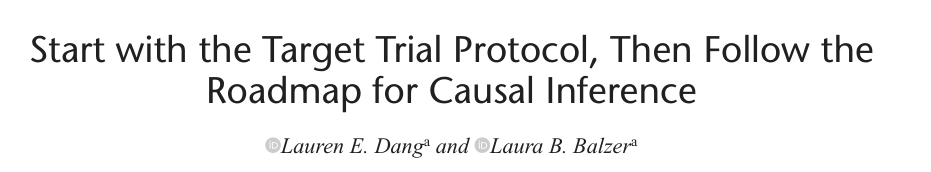
\includegraphics[width=0.9\linewidth]{art/Dang}

\end{figure}

\end{frame}

% ----------------------------------------
\begin{frame}{The Causal Roadmap: A 9-Step Framework}
  \small
  \begin{columns}[c]
    \begin{column}{0.30\textwidth}
      \textbf{From Petersen \& van der Laan (2014) and Dang et al.\ (2023)}

      \vspace{0.8cm}
      \textcolor{accent}{\textbf{Key:}} Complete most steps \emph{before}
      looking at treatment-outcome associations!
    \end{column}
    \begin{column}{0.66\textwidth}
      \centering
      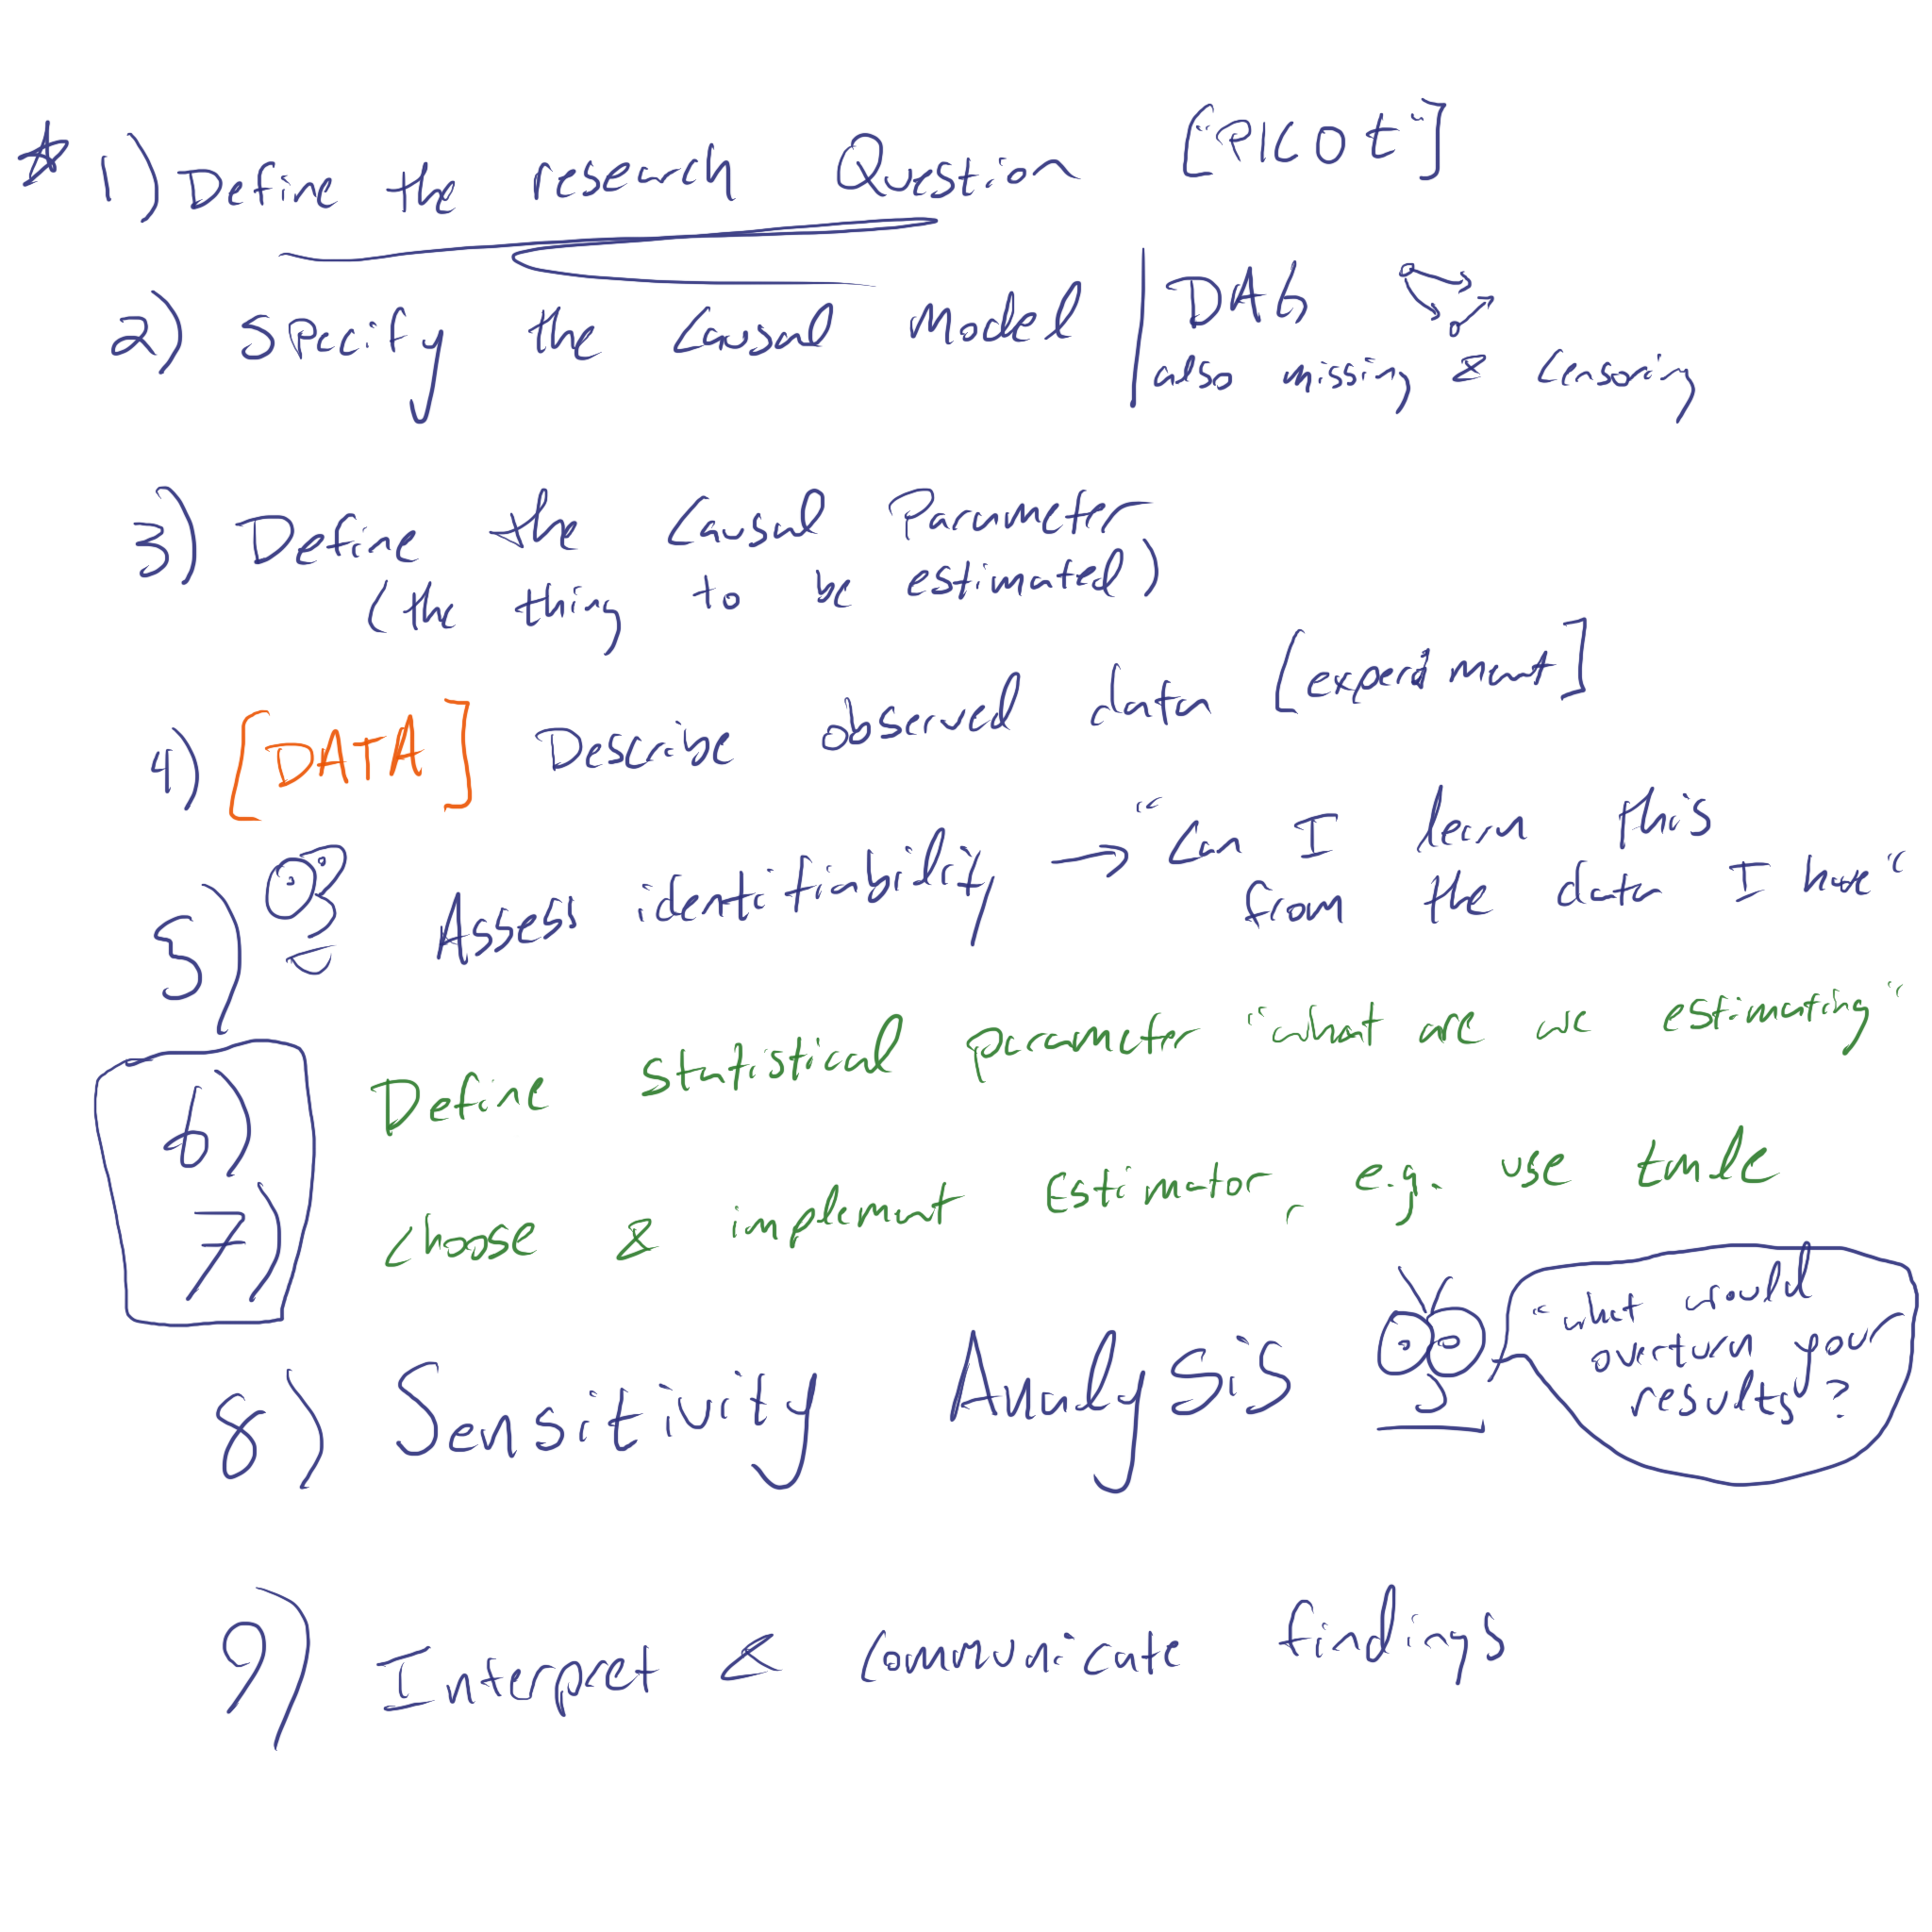
\includegraphics[height=0.70\textheight,keepaspectratio]{art/roadmap9.png}
    \end{column}
  \end{columns}
\end{frame}

\section{Phase 1: Defining the Causal Question (Steps 1--3)}

% ----------------------------------------
\begin{frame}{Step 1: Specify the Research Question}
  \small
  \textbf{A complete research question should specify:}
  \begin{itemize}
    \item \textbf{Target population:} Who is included?
    \item \textbf{Exposure/intervention:} What treatments are compared?
    \item \textbf{Outcome:} What is measured and when?
    \item \textbf{Time horizon:} Follow-up period
    \item \textbf{Context:} Setting and data source
  \end{itemize}

\end{frame}

% ----------------------------------------
\begin{frame}{Step 1 Applied: Pneumonia Vaccine}
  \small
  \begin{columns}[T]
    \begin{column}{0.48\textwidth}
      \textbf{Target population:}
      \begin{itemize}
        \item Adults in health system Y; age centered near 65
      \end{itemize}
      \vspace{0.3em}

      \textbf{Exposure ($A$):}
      \begin{itemize}
        \item $A=1$: Pneumococcal vaccination at baseline
        \item $A=0$: No vaccination at baseline
      \end{itemize}
      \vspace{0.3em}

      \textbf{Outcome ($Y$):}
      \begin{itemize}
        \item Pneumonia hospitalization within 1 year
      \end{itemize}
    \end{column}
    \begin{column}{0.48\textwidth}
      \textbf{Time horizon:}
      \begin{itemize}
        \item Baseline vaccination, 12-month follow-up
      \end{itemize}
      \vspace{0.3em}

      \textbf{Context:}
      \begin{itemize}
        \item Fixed synthetic health-system cohort
      \end{itemize}
      \vspace{0.3em}

      \textbf{Decision context:}
      \begin{itemize}
        \item What would vaccination versus no vaccination change in this cohort?
      \end{itemize}
    \end{column}
  \end{columns}
\end{frame}



% ----------------------------------------
\begin{frame}{Step 2: Specify a Causal Model}
  \small
  \textbf{Represent assumptions about how the world works:}
  \begin{itemize}
    \item Relationships between exposure, outcome, and covariates
    \item Potential confounders (baseline or time-varying)
    \item Possible sources of selection or measurement bias
  \end{itemize}
  \vspace{0.5em}

  \textbf{The na\"ive (incorrect) implicit model:}
  \begin{center}
    \begin{tikzpicture}[scale=0.8]
      \node[draw, circle, fill=green!20] (A) at (0,0) {$A$};
      \node[draw, circle, fill=orange!20] (Y) at (3,0) {$Y$};
      \draw[->, thick] (A) -- (Y);
    \end{tikzpicture}
  \end{center}
  \vspace{0.3em}

  This is actually how we'd depict if A was randomized (notice A isn't `listening' to any other variables in this example)

\end{frame}

% ----------------------------------------
\begin{frame}{Step 2 Applied: The Correct DAG (Directed Acyclic Graph)}
  \small
  \textbf{Clinical practice creates confounding by indication:}
  \vspace{0.3em}

  \begin{columns}[T]
    \begin{column}{0.55\textwidth}
      \begin{center}
        \begin{tikzpicture}[scale=1.0]
          \node[draw, circle, fill=accent!20] (W) at (1.5,1.5) {$W$};
          \node[draw, circle, fill=green!20] (A) at (0,0) {$A$};
          \node[draw, circle, fill=orange!20] (Y) at (3,0) {$Y$};

          \draw[->, thick] (W) -- (A);
          \draw[->, thick] (W) -- (Y);
          \draw[->, thick] (A) -- (Y);
        \end{tikzpicture}
      \end{center}
      \vspace{0.3em}

      \textbf{Variables:}
      \begin{itemize}
        \item $W$: Age, prior pneumonia, prior vaccination
        \item $A$: Vaccination status
        \item $Y$: Pneumonia hospitalization
      \end{itemize}
    \end{column}
    \begin{column}{0.42\textwidth}
      \textbf{Backdoor path:}
      \[
        A \leftarrow W \rightarrow Y
      \]
      \vspace{0.3em}

      \textbf{Interpretation:}
      \begin{itemize}
        \item Baseline risk history predicts vaccination
        \item Same factors increase pneumonia risk
        \item $W$ confounds the $A \to Y$ relationship
      \end{itemize}
    \end{column}
  \end{columns}
\end{frame}

% ----------------------------------------
\begin{frame}{Step 3: Define the Causal Estimand}
  \small
  \textbf{Translate the question into a formal causal estimand:}
  \vspace{0.5em}

  For a binary exposure, a common target is the \textbf{Average Treatment Effect (ATE):}
  \[
    \text{ATE} = E[Y^{(1)}] - E[Y^{(0)}]
  \]
  where $Y^{(1)}$ and $Y^{(0)}$ are potential outcomes under vaccination vs.\ no vaccination.
  \vspace{0.5em}

  \textbf{Other common causal estimands:}
  \begin{itemize}
    \item Risk ratio, odds ratio, hazard ratio
    \item Subgroup-specific effects (CATE)
    \item Effects over time (survival curves)
  \end{itemize}
  \vspace{0.5em}

  \textcolor{accent}{\textbf{For our example:}} ATE = causal reduction in 1-year pneumonia risk due to vaccination, in the synthetic adult cohort.
\end{frame}

\section{Phase 2: Connecting to Data (Steps 4--6)}

% ----------------------------------------
\begin{frame}{Step 4: Describe the Observed Data}
  \small
  \textbf{Connect the causal question to available data:}
  \begin{itemize}
    \item What variables are measured? When? How?
    \item Are there missing data or censoring mechanisms?
    \item Does the data structure match the causal model?
  \end{itemize}
  \vspace{0.25em}

  \textbf{For the fixed synthetic vaccine example:}
  \begin{itemize}
    \item $W$: Age, prior pneumonia, and prior vaccination at baseline
    \item $A$: Vaccination status at baseline
    \item $Y$: Pneumonia hospitalization within 12 months
  \end{itemize}
  \vspace{0.2em}

  \textbf{Data structure:} \quad $O = (W, A, Y)$ for each person
  \vspace{0.2em}

  \textcolor{accent}{\textbf{Key question:}} Do we have all common causes in $W$? This determines identifiability.
\end{frame}

% ----------------------------------------
\begin{frame}{Step 5: Assess Identifiability}
  \small
  \textbf{Can we answer the causal question from observed data?}
  \vspace{0.2em}

  \textbf{Core assumptions required:}
  \begin{itemize}
    \item \textbf{Consistency:} Observed $Y$ equals $Y^{(a)}$ when $A=a$
    \item \textbf{Exchangeability:} $Y^{(a)} \perp\!\!\!\perp A \mid W$ (no unmeasured confounding)
    \item \textbf{Positivity:} $P(A=a \mid W) > 0$ for all $W$ and $a$
  \end{itemize}
  \vspace{0.2em}

  \textbf{For the vaccine example:} if $W$ (age, prior pneumonia, prior vaccination) blocks all
  backdoor paths $\rightarrow$ \textbf{identifiable}; with unmeasured
  confounders $\rightarrow$ \textbf{not identifiable} without further
  assumptions.
  \vspace{0.2em}

  \textcolor{accent}{\textbf{The identification gap:}} Step 5 characterizes
  the assumptions connecting the causal question to an estimable
  observed-data quantity; it does not quantify bias.
\end{frame}

% ----------------------------------------
\begin{frame}{Step 6: Define the Statistical Estimand}
  \small
  \setlength{\abovedisplayskip}{4pt}\setlength{\belowdisplayskip}{4pt}
  \textbf{Under identifiability, express the causal estimand in observed data:}

  \textbf{Causal estimand:} $\psi = E[Y^{(1)}] - E[Y^{(0)}]$

  \textbf{Statistical estimand:}
  \[
    \psi = \sum_{w} \left( E[Y \mid A=1, W=w] - E[Y \mid A=0, W=w] \right) P(W=w)
  \]

  \textbf{Interpretation:}
  \begin{itemize}
    \item For each covariate profile $w$, compare expected outcomes,
      weighted by the population distribution of $W$
    \item This is the \textbf{standardized} (G-computed) effect
  \end{itemize}
  \vspace{0.2em}

  \textcolor{accent}{\textbf{Step 6 bridges theory and practice}} --- defines exactly what to estimate.
\end{frame}

\section{Phase 3: Estimation \& Interpretation (Steps 7--9)}

% ----------------------------------------
\begin{frame}{Step 7: Choose and Implement an Estimator}
  \small
  \textbf{Select a method to estimate the statistical estimand:}
  \vspace{0.3em}

  \begin{columns}[T]
    \begin{column}{0.48\textwidth}
      \textbf{Common estimators:}
      \begin{itemize}
        \item Outcome regression (G-computation)
        \item Propensity score methods (IPTW, matching)
        \item Doubly-robust: TMLE, AIPW
        \item Machine learning + causal inference
      \end{itemize}
    \end{column}
    \begin{column}{0.48\textwidth}
      \textbf{Key considerations:}
      \begin{itemize}
        \item Flexibility for nonlinear relationships
        \item Robustness to model misspecification
        \item Valid confidence intervals
        \item Computational feasibility
      \end{itemize}
    \end{column}
  \end{columns}
  \vspace{0.6em}

  \textbf{Best practice:} prespecify the causal question, adjustment set,
  estimator, and sensitivity plan. Outcome-model fitting and tuning may use
  \(Y\); do not choose the analysis based on the observed treatment-effect
  result.
  \vspace{0.25em}

  \textcolor{accent}{\textbf{Estimation:}} When appropriate, prefer
  doubly-robust methods (TMLE, AIPW). \textcolor{accent}{\textbf{Module G}}
  continues this example with a live TMLE walkthrough.
\end{frame}

\begin{frame}{Preview TMLE}
\begin{figure}
	\centering
	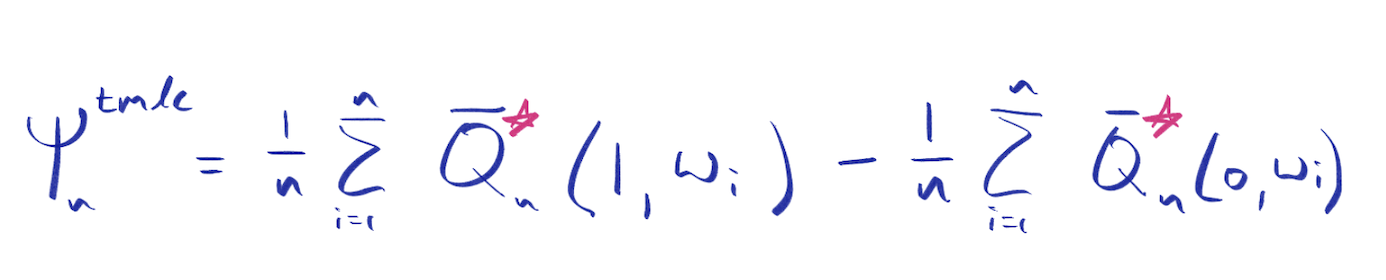
\includegraphics[width=0.7\linewidth]{art/tmle}
\end{figure}


\end{frame}

% ----------------------------------------
\begin{frame}{Step 8: Conduct Sensitivity Analyses}
  \small
  \textbf{How robust are conclusions to assumption violations?}
  \vspace{0.1em}

  \textbf{Key sensitivity analyses:}
  \begin{itemize}
    \item \textbf{Unmeasured confounding:} E-value, bias factor analysis
    \item \textbf{Outcome misclassification:} Impact of PPV/sensitivity
    \item \textbf{Selection bias:} Informative censoring scenarios
    \item \textbf{Negative controls:} Exposure/outcome falsification tests
  \end{itemize}
  \vspace{0.1em}

  \textbf{E-value example:}
  \begin{itemize}
    \item ``How strong would unmeasured confounding need to be to explain away our finding?''
    \item Provides calibrated measure of robustness
  \end{itemize}
  \vspace{0.1em}

  \textcolor{accent}{\textbf{Prespecify:}} Plan sensitivity analyses before examining results.
\end{frame}

% ----------------------------------------
\begin{frame}{Step 9: Interpret Results in Context}
  \small
  \textbf{Translate findings back to the original question:}
  \vspace{0.5em}

  \begin{itemize}
    \item \textbf{Primary result:} Point estimate and 95\% CI
    \item \textbf{Interpretation level:} Causal effect, association, or ``evidence consistent with''?
    \item \textbf{Limitations:} What could bias results? What remains unknown?
    \item \textbf{Applicability:} Does this generalize to other populations?
  \end{itemize}
  \vspace{0.5em}

  \textcolor{red}{\textbf{Match language to evidence:}}
  \begin{itemize}
    \item Strong assumptions satisfied $\rightarrow$ ``The vaccine \emph{reduced} pneumonia risk''
    \item Assumptions uncertain $\rightarrow$ ``Evidence \emph{suggests} a protective effect''
  \end{itemize}
  \vspace{0.5em}

  \textcolor{accent}{\textbf{Honesty matters:}} Overstating causal claims undermines credibility.
\end{frame}

\begin{frame}{Nine Literature Steps Map to Eight Navigator Steps}
  \scriptsize
  Navigator groups the work; it does not remove a scientific decision.
  \vspace{0.25em}

  \renewcommand{\arraystretch}{1.18}
  \begin{center}
    \begin{tabular}{@{}p{0.41\textwidth}p{0.49\textwidth}@{}}
      \textbf{Nine-step literature roadmap} &
      \textbf{Eight-step Causal Navigator} \\
      \hline
      1.\ Research question + 3.\ causal estimand &
      1.\ Define the causal question + contrast \\
      2.\ Causal model &
      2.\ Specify the causal model \\
      4.\ Observed data &
      3.\ Consider the observed data \\
      5.\ Identifiability &
      4.\ Assess identifiability \\
      6.\ Statistical estimand &
      5.\ Define the statistical estimand \\
      7.\ Estimator &
      6.\ Choose the estimator \\
      8.\ Sensitivity analysis &
      7.\ Plan sensitivity analyses \\
      9.\ Interpretation &
      8.\ Record results and interpretation \\
    \end{tabular}
  \end{center}

  \vspace{0.25em}
  \textcolor{accent}{\textbf{Module F uses Navigator numbering:}}
  question and causal contrast are recorded together in Step 1; later labels
  shift by one.
\end{frame}

\section{The Interactive Tool}

\begin{frame}{A good idea whose time has come}

\begin{figure}
	\centering
	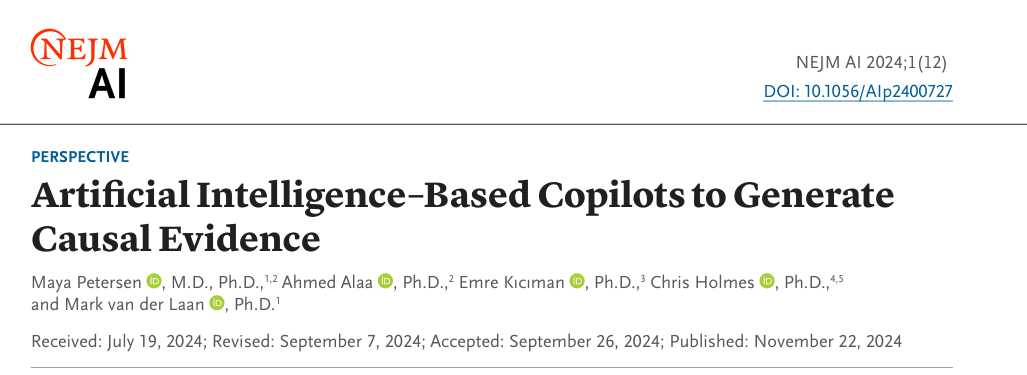
\includegraphics[width=0.8\linewidth]{art/copilots}
\end{figure}


\end{frame}

\begin{frame}{A good idea whose time has come}

	\begin{figure}
		\centering
		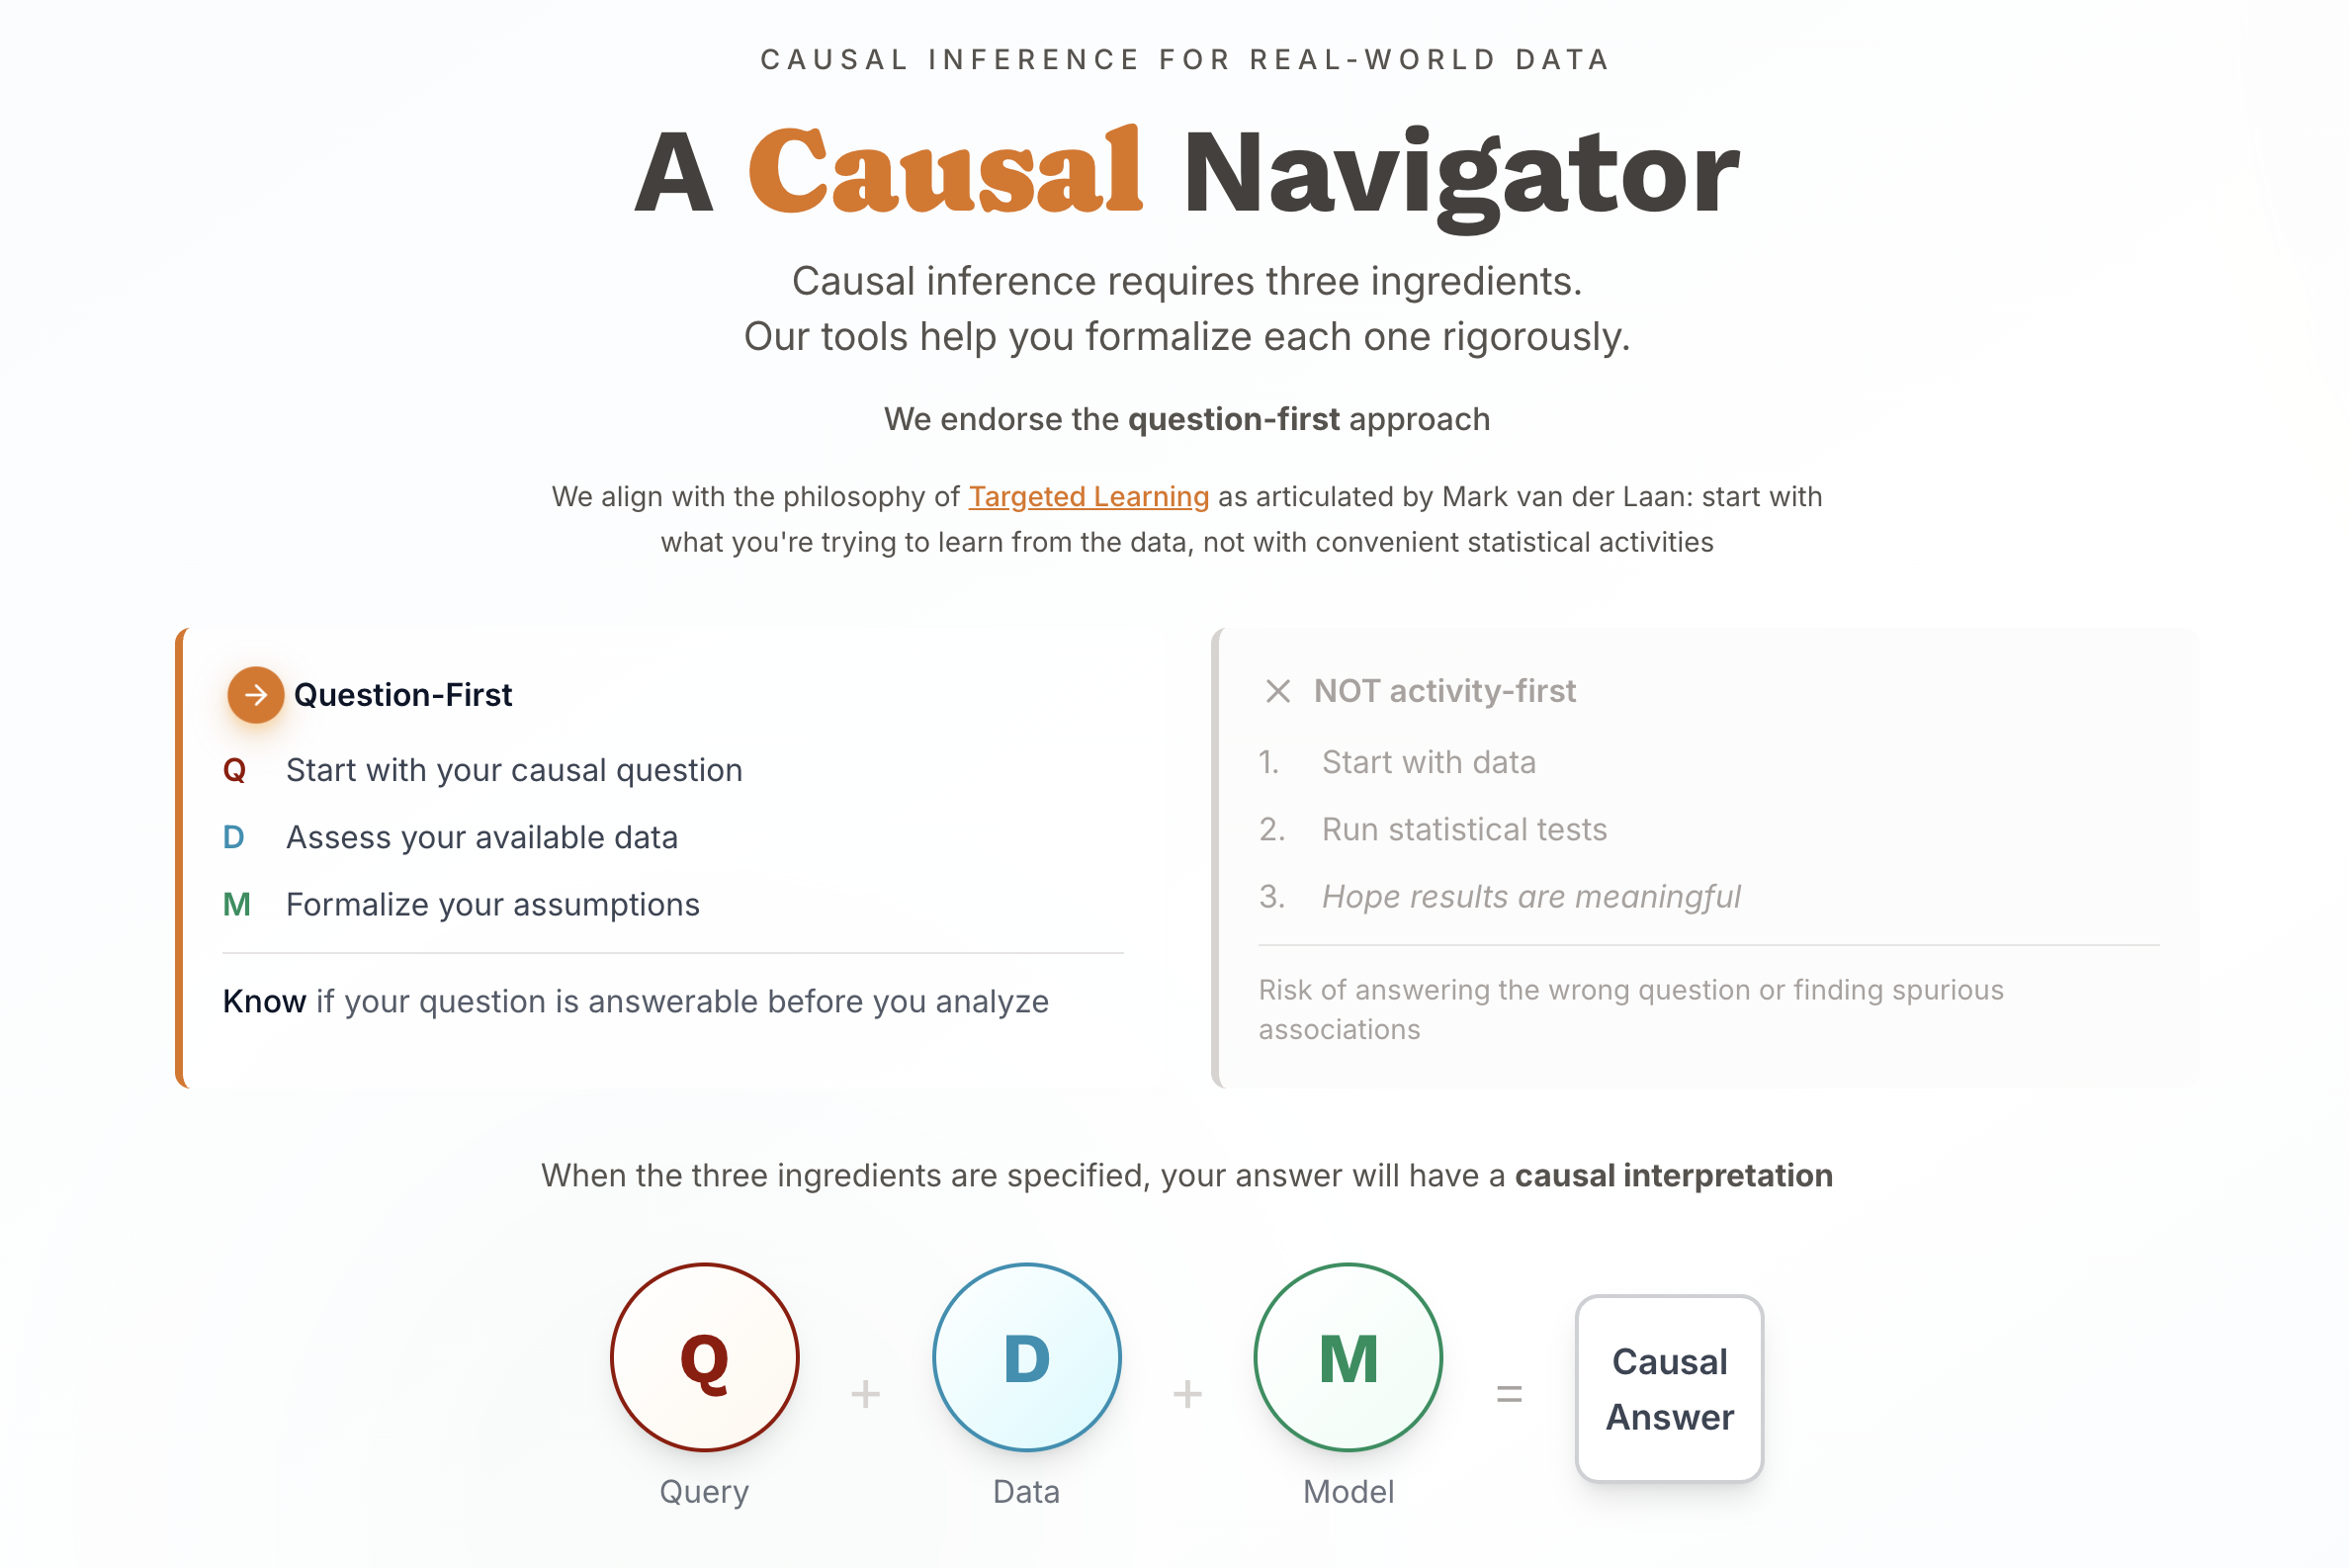
\includegraphics[height=0.68\textheight,keepaspectratio]{art/navigator}
	\end{figure}


\end{frame}


% ----------------------------------------
\begin{frame}{The Causal Roadmap App - Causal Navigator}
  \small
  \textbf{An interactive web tool for designing rigorous causal studies}
  \vspace{0.2em}

  \begin{columns}[T]
    \begin{column}{0.55\textwidth}
      \textbf{Features:}
      \begin{itemize}
        \item guided workflow
        \item Structured form fields at each step
        \item Worked examples throughout
        \item AI Copilot for guidance (optional)
        \item Export to Markdown/text
        \item Save \& load study designs
      \end{itemize}
    \end{column}
    \begin{column}{0.42\textwidth}
      \textbf{Purpose:}
      \begin{itemize}
        \item Document assumptions
        \item Structure your thinking
        \item Communicate with collaborators
        \item Create audit trail
        \item Support regulatory submissions
      \end{itemize}
    \end{column}
  \end{columns}
  \vspace{0.2em}
  \centering
  \url{https://navigator.tao-rwd.com/}
  \quad\textcolor{accent}{\textbf{Module F:}} live walkthrough with a prepared study.
\end{frame}

\section{Summary}

% ----------------------------------------
\begin{frame}{Why Use a Structured Workflow?}
  \small
  \begin{columns}[T]
    \begin{column}{0.48\textwidth}
      \textcolor{green!60!black}{\textbf{With the Roadmap:}}
      \begin{itemize}
        \item Explicit assumptions
        \item Clear audit trail
        \item Design separated from analysis
        \item Transparent communication
        \item Supports preregistration
        \item Facilitates collaboration
      \end{itemize}
    \end{column}
    \begin{column}{0.48\textwidth}
      \textcolor{red!70!black}{\textbf{Without structure:}}
      \begin{itemize}
        \item Hidden assumptions
        \item Ad-hoc decisions
        \item Outcome-driven analysis
        \item ``Garden of forking paths''
        \item Difficult to replicate
        \item Hard to critique
      \end{itemize}
    \end{column}
  \end{columns}
  \vspace{1em}
  \centering
  \Large
  \textbf{Structure enables both \textcolor{accent}{rigor} and \textcolor{accent}{transparency}}
\end{frame}

% ----------------------------------------
\begin{frame}{Module D Summary}
  \small
  \textbf{The 9-step Causal Roadmap:}
  \vspace{0.3em}

  \begin{enumerate}
    \item \textbf{Research question} --- population, exposure, outcome, timing
    \item \textbf{Causal model} --- DAG representing assumptions
    \item \textbf{Causal estimand} --- formal target quantity ($E[Y^{(1)}] - E[Y^{(0)}]$)
    \item \textbf{Observed data} --- what's measured and how
    \item \textbf{Identifiability} --- can we answer the question?
    \item \textbf{Statistical estimand} --- observable quantity equal to causal effect
    \item \textbf{Estimator} --- method to compute the estimate
    \item \textbf{Sensitivity analysis} --- robustness to assumptions
    \item \textbf{Interpretation} --- conclusions in context
  \end{enumerate}
  \vspace{0.3em}

  \textcolor{accent}{\textbf{Next:}} Module E --- Audit-First AI
\end{frame}

% ----------------------------------------
\begin{frame}{}
  \vfill
  \centering
  \Large
  \textbf{Questions?}

  \vspace{2em}

  \normalsize
  Next module: \textbf{Audit-First AI}

  \vspace{1em}

  \small
  Auditing an AI-generated roadmap field: accept, correct, or reject
  \vfill
\end{frame}

% ----------------------------------------
\begin{frame}{References}
  \footnotesize
  \textbf{Foundational papers:}
  \begin{itemize}
    \item Petersen \& van der Laan (2014). Causal models and learning from data. \textit{Epidemiology}.
    \item Dang et al.\ (2023). A causal roadmap for generating high-quality RWE. \textit{J Clin Transl Sci}.
    \item Hern{\'a}n \& Robins (2016). Using big data to emulate a target trial. \textit{Am J Epidemiol}.
  \end{itemize}
  \vspace{0.3em}

  \textbf{Additional resources:}
  \begin{itemize}
    \item ICH E9(R1) Addendum on Estimands (2019)
    \item Hern{\'a}n \& Robins (2020). \textit{Causal Inference: What If}. Chapman \& Hall/CRC.
  \end{itemize}
\end{frame}

\end{document}
